\subsection{Die Wissenstr�gerschnittstelle}
Bei der Wissenstr�gerschnittstelle handelt es sich um eine Methode zur Datenerfassung, die einen direkten Wissenstransfer zwischen einem Wissenstr�ger und dem Expertensystem erm�glicht. Da die Daten manuell eingegeben und maschinell verarbeitet werden, bezeichnet man die Wissenstr�gerschnittstelle als semi-automatisierte Wissenserfassungsmethode. Im Folgenden wird ein Anwendungsbeispiel aus der Praxis betrachtet und in Bezug auf die Erkenntnisse bei der Entwicklung und dem Einsatz erl�utert.\\
Das Praxisbeispiel wird in der \cite{gebus2009} vorgestellt und bezieht sich auf die Wissenserfassung aus der Produktion eines Elektrotechnikunternehmens. In der Fallstudie wird ein bereits bestehendes \ac{DSS} betrachtet, das die F�hrungskr�fte bei den Entscheidungen von nicht-strukturieren Problemen in der Produktion unterst�tzt \cite[S.94]{gebus2009}. Das DSS verf�gt bereits �ber eine Datenbank, die allerdings nur Daten von Produkteigenschaften enth�lt. Die eigentlichen Prozesse werden allerdings von Experten gesteuert, die mithilfe des Erfahrungswissens St�rungen in der Produktion beseitigen. Dieses Erfahrungswissen �ber St�rungen wird im System nicht erfasst. Als Folge hat die Unternehmensf�hrung einen begrenzten �berblick �ber die Situation in der Produktionsabteilung. Au�erdem besteht die Gefahr, dass das spezifische Expertenwissen verloren geht, falls der Wissenstr�ger das Unternehmen verl�sst.\\
Die Zielsetzung von \cite{gebus2009} ist die Erfassung des Expertenwissens aus der Produktion und die Integration dieses Wissens in die Entscheidungsprozesse auf der Organisationsebene. Im Gro�en und Ganzen handelt es sich um die Gestaltung eines wissensbasierten Systems. Um das Wissen aus der Produktionsabteilung zu erschlie�en, wollen Gebus und Leivisk{\"a} das System um eine Schnittstelle (User Interface) f�r Anlagenbediener erweitern. Die Entwicklung der Schnittstelle l�sst sich wie folgt beschreiben:
\begin{itemize}
\item Die f�r die Schnittstelle relevante Zielgruppe wird definiert.
\item Ausgehend von der Zielgruppe werden funktionale und nicht-funktionale Anforderungen an die Schnittstelle festgelegt.
\item Anschlie�end wird die Schnittstelle evaluiert.
\end{itemize}
Im ersten Schritt definieren Gebus und Leivisk{\"a} die bestehenden Nutzergruppen des gesamten Systems \cite[S.97]{gebus2009}:
\begin{itemize}
\item Anlagenbediener (Experte), der sein Wissen zu den St�rungen mittels der Wissenstr�gerschnittstelle in die Datenbank eingibt.
\item Administrator, der das gesamte DSS verwaltet und bei Bedarf die Systemeinstellungen anpasst.
\item Qualit�tsabteilung, die die St�rungsstatistik analysiert, eine Qualit�tsr�ckmeldung an die Produktion und einen Bericht an die F�hrungskraft �bermittelt.
\item F�hrungskraft, die eine umfangreiche �bersicht von der Qualit�tsabteilung erh�lt und davon ausgehend Entscheidungen zur Prozessoptimierung trifft.
\end{itemize}
Im Rahmen der Fallstudie ist die Nutzergruppe der Anlagenbediener relevant, wobei das System jeder Nutzergruppe eine geeignete Benutzerschnittstelle zur Verf�gung stellt. Schematisch l�sst sich die Struktur und die Informationsfl�sse im DSS in der Abbildung \ref{dss_gebus} vereinfacht nachbilden.
\begin{figure}[H] 
	\centering
	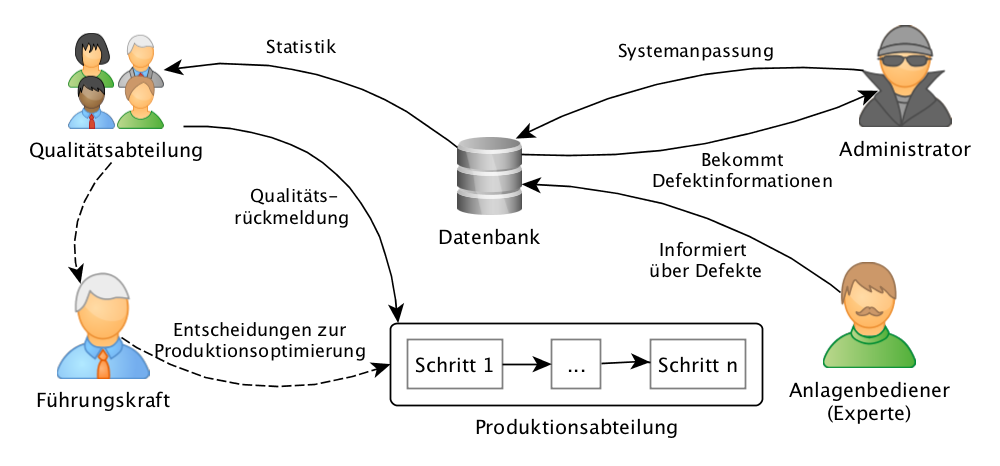
\includegraphics[width=0.9\textwidth]{images/dss_gebus.png}
	\caption{Die Struktur und die Informationsfl�sse im DSS, \cite[S.98]{gebus2009}}
	\label{dss_gebus}
\end{figure} 
Die Autoren betonen, dass die Expertenschnittstelle einfach und intuitiv wie m�glich gehalten wurde, um die Dateneingabe zu einer allt�glichen T�tigkeit zu machen \cite[S.97]{gebus2009}. Im Hinblick auf die nicht-funktionalen Anforderungen werden beispielsweise Einstellungen und Maschinenbilder vom Administrator vorkonfiguriert und automatisch beim Hochfahren des Systems geladen. Die funktionalen Anforderungen umfassen die Erfassung einer St�rung durch die Auswahl passender Maschine und das Markieren der betroffenen Stelle. Darauffolgend wird eine Vorlage mit m�glichen Ursachen zur Auswahl angezeigt. Zus�tzlich gibt es ein Feld zur Freitexteingabe, wenn die vorliegende St�rung im System noch nicht vorhanden ist \cite[S.99]{gebus2009}.




